\documentclass[11pt,twoside,a4paper]{article}
\usepackage[margin=2cm]{geometry}
\usepackage{titling}
\usepackage{url}
\usepackage[hidelinks]{hyperref}
\usepackage{natbib}
%\usepackage[font=small,labelfont=bf]{caption}
\usepackage{array}
\usepackage[version=4]{mhchem}

\newcommand{\doi}[1]{\href{http://dx.doi.org/#1}{doi:#1}}

% color
\RequirePackage{graphicx}
\RequirePackage{xcolor}
\definecolor{color1}{rgb}{0.0,0.56,0.35}
\usepackage{sectsty}
\allsectionsfont{\color{color1}\normalfont}

% automatic loading of latin modern fonts if present on the system
\IfFileExists{lmodern.sty}
  {\RequirePackage[T1]{fontenc}\RequirePackage{lmodern}}
  {}

% symbols like \Telefon, \Mobilefone, \Letter and \Email
\RequirePackage{marvosym}

\newcolumntype{L}[1]{>{\raggedright\let\newline\\\arraybackslash\hspace{0pt}}m{#1}}
\newcolumntype{C}[1]{>{\centering\let\newline\\\arraybackslash\hspace{0pt}}m{#1}}
\newcolumntype{R}[1]{>{\raggedleft\let\newline\\\arraybackslash\hspace{0pt}}m{#1}}

\posttitle{\par\end{center}}
\predate{}
\postdate{}
\date{}
\preauthor{\begin{center}}
\postauthor{\par\end{center}\vspace{-0.5em}}
\setlength{\droptitle}{-60pt}

%   other symbols
\newcommand*{\listitemsymbol}{\labelitemi~}
\newcommand*{\addresssymbol}{}
\newcommand*{\mobilesymbol}{\Mobilefone~}
\newcommand*{\phonesymbol}{\Telefon~}
\newcommand*{\faxsymbol}{\FAX~}
\newcommand*{\emailsymbol}{\Letter~}
\newcommand*{\homepagesymbol}{{\Large\ComputerMouse}~}


\title{}

\begin{document}

%\maketitle

\vspace{-5em}

\begin{center}
\begin{minipage}[b]{0.53\textwidth}
  \raggedright
  \Huge{Robert Myhill} \par
  \LARGE{\color{color1} Postdoctoral Researcher} \par
  \vspace{0.5em}
\end{minipage}%
\begin{minipage}[b]{0.33\textwidth}
  \raggedleft
  \scriptsize \it \color{gray}
  School of Earth Sciences, \\
  University of Bristol, \\
  BS8 1RJ, UK\\
  \phonesymbol +44 (0) 117 33 15141 \\
  \mobilesymbol +44 (0) 778 334 2237 \\
  \emailsymbol \href{mailto:bob.myhill@bristol.ac.uk}{bob.myhill@bristol.ac.uk} \\
  \homepagesymbol \url{https://bobmyhill.github.io}\\
\end{minipage}%
\begin{minipage}[b]{0.02\textwidth}
  \raggedleft \textcolor{white}{.}
\end{minipage}%
\begin{minipage}[b]{0.12\textwidth}
  \raggedleft
      {%
        \color{color1}
        \setlength{\fboxsep}{1.pt}%
        \setlength{\fboxrule}{0.8pt}%
        \fbox{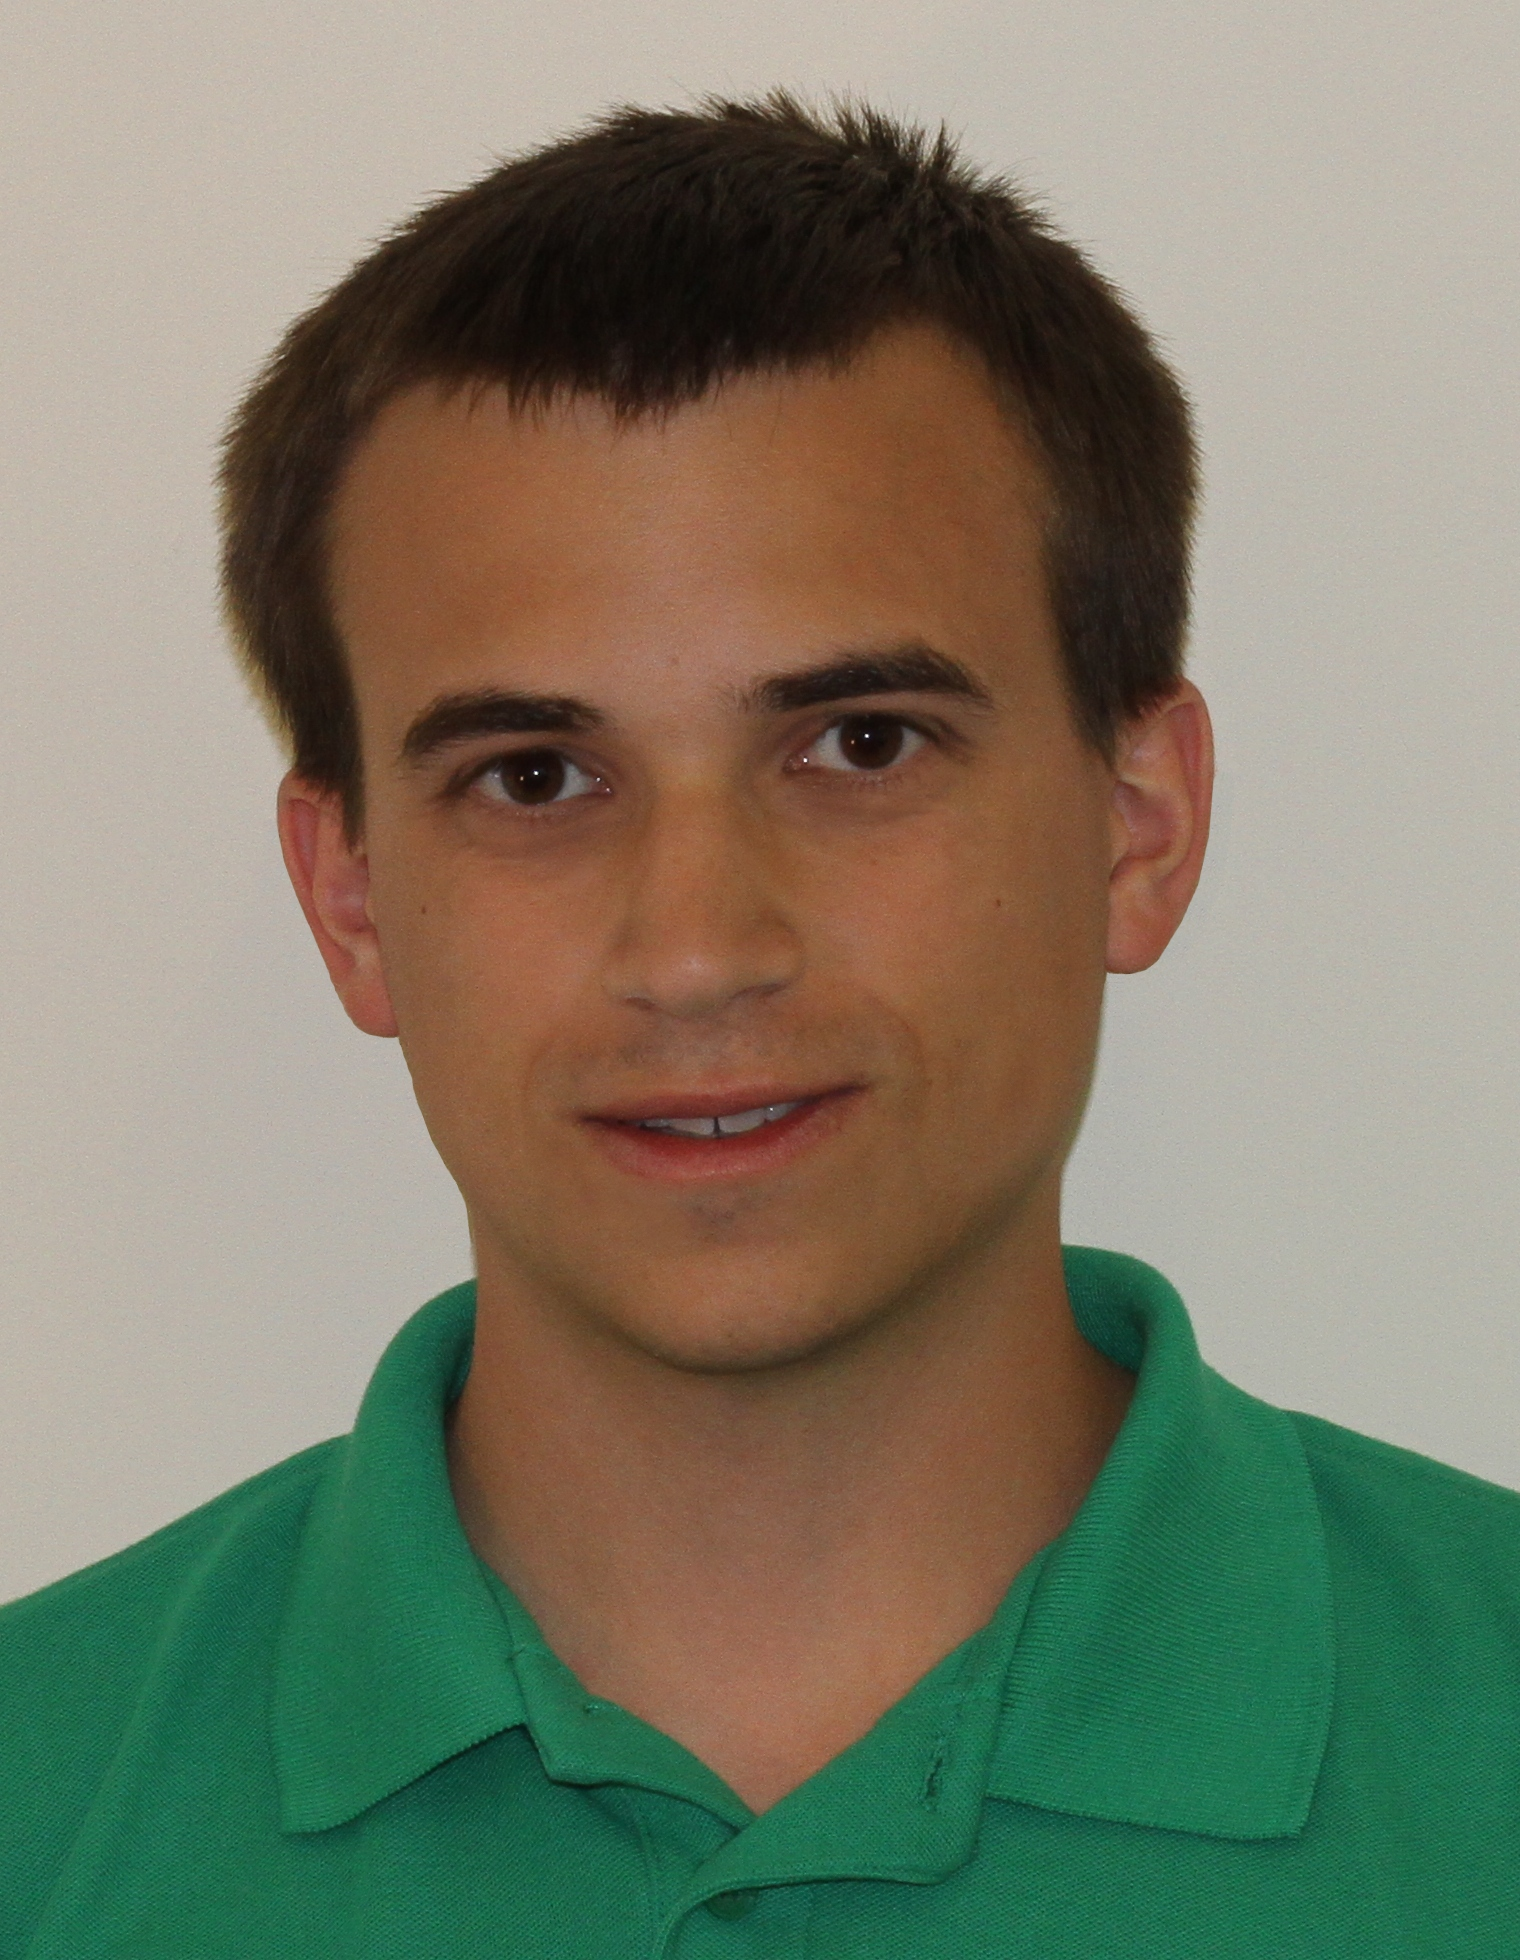
\includegraphics[width=\linewidth]{photo/photo}}%
      }%
\end{minipage}
\end{center}


\vspace{0.2em}

\subsection*{PROFESSIONAL EXPERIENCE}
\vspace{-0.5em}
\begin{table}[!h]
\centering
\begin{tabular}{L{2cm} L{10.5cm} L{4.5cm}}
2021-present & NERC Large Grant Co-Researcher Investigator \newline \emph{Mantle Convection Constrained} & University of Bristol \vfill \\
2017-2021 & UK Space Agency Postdoctoral Research Fellow \newline \emph{The thermochemical state and evolution of Mars' deep interior} & University of Bristol \vfill \\
2016 \vfill & Postdoctoral Research Associate \newline \emph{Preparation for the InSight Mission} & University of Bristol \vfill \\
2015 \vfill & Postdoctoral Researcher \newline \emph{Thermodynamics of core formation} & Bayerisches Geoinstitut \vfill \\
2013-2014 \vfill & Alexander von Humboldt Research Fellow \newline \emph{High pressure experimental petrology} & Bayerisches Geoinstitut \vfill \\
2012 \vfill & Visiting Scientist \newline \emph{High pressure experimental petrology} & Bayerisches Geoinstitut \vfill
\end{tabular}
\end{table}
\vspace{-1.5em}

\subsection*{EDUCATION}
\vspace{-0.5em}
\begin{table}[!h]
\centering
\begin{tabular}{L{2cm} L{10.5cm} L{4.5cm}}
2012 \vfill & PhD Geophysics \newline \emph{The Mechanisms of Deep Earthquakes} & University of Cambridge\vfill \\
2008 \vfill & MSci Natural Sciences (1/32 in class) \newline \emph{Earth Sciences} & University of Cambridge \vfill\\
2007 \vfill & MA Natural Sciences (1/36 in class) \newline \emph{Geology (plus Physics, Maths and Chemistry)} & University of Cambridge \vfill
\end{tabular}
\end{table}
\vspace{-1.5em}

\subsection*{SELECTED HONOURS AND AWARDS}

\vspace{-0.5em}
\begin{table}[!h]
\centering
\begin{tabular}{L{2cm} L{13cm} L{2cm}}
2017-2020 & UK Space Agency Aurora Postdoctoral Fellowship (302k GBP) & \\
2013-2014 & Alexander von Humboldt Research Fellowship for Postdoctoral Researchers & \\
2011 & Outstanding Student Poster Award, Geodynamics Division (European Geophysical Union General Assembly) & \\
2010 & The Kingsley Bye-Fellowship. Magdalene College, Cambridge & \\
2008 & The Hugo de Balsham Prize for Exceptional Academic Distinction & \\
 & The Harkness Scholarship (first-placed Finalist in Geological Sciences, University of Cambridge) & \\
 & The Huppert Prize in Geophysics &  \\
2007 & The Henry Wilkinson Cookson Senior Scholarship in Natural Sciences &
\end{tabular}
\end{table}
\vspace{-1.5em}

\clearpage
\subsection*{TEACHING EXPERIENCE}
\vspace{-0.5em}
\begin{table}[!h]
\centering
\begin{tabular}{L{2cm} L{13cm} L{2cm}}
  2019--2020 & Lecturer in \emph{Non-Renewable Resources} (University of Bristol) & \\
  2019 & Organiser, Avon Gorge Field Trip (University of Bristol) &\\
  2018 & Field demonstrator, Arran Field Trip (University of Bristol) & \\
  2017 \vfill & Guest lecturer on the subjects of \emph{high pressure melting} and the \emph{InSight Mission} (USTC, China) & \\
  2017-2018 & Guest lecturer on \emph{subduction} and \emph{Mars exploration} (University of Bristol) & \\
  2016-2018 & Field demonstrator, Avon Gorge Field Trip (University of Bristol) & \\
  2008-2011 & Field demonstrator, Sedbergh Field Trip (University of Cambridge) & \\
  2009 & Field demonstrator, Arran Field Trip (University of Cambridge) &
\end{tabular}
\end{table}
\vspace{-1.5em}

\subsection*{SKILLS}
\begin{itemize}
\item Postdoctoral experience in high pressure experimental petrology on melts, silicate and oxide phases, using piston cylinder and multi-anvil apparatus.
\item Analytical experience includes EPMA, SEM, XRD, M\"ossbauer, Raman and ERDA techniques.
\item Fluent in the Python programming language. Competent in C++, BASH and HTML scripting. Basic knowledge of FORTRAN and the OpenGL API.
\item Over 400 hours experience with \href{http:www.metamorph.geo.unimainz.de/thermocalc/}{THERMOCALC}, and a competent user of \href{http:www.perplex.ethz.ch/}{Perple\_X} thermodynamic software.
\item Competent user of \href{http://www.latex-project.org/}{\LaTeX}, Microsoft and Serif Office programs.
\item Experience in waveform modelling, including receiver function construction, directivity and focal mechanism analysis and relocation routines.
\end{itemize}

\subsection*{SELECTED COMMUNITY ROLES}
\begin{itemize}
\item Session convener at AGU Fall Meeting on seismology (2012), mineral physics (2015) and planetary sciences (2016).
\item Reviewer for \emph{American Mineralogist}, \emph{Contributions to Mineralogy and Petrology}, \emph{Earth and Planetary Science Letters}, \emph{G-cubed}, \emph{GeoResJ}, \emph{Minerals}, \emph{Science Advances}, \emph{SoftwareX} and \emph{Solid Earth}, amongst others. %\emph{The Journal of Mineralogical and Petrological Sciences}.
\item Chapter editor for Geochemical Perspectives.
\item Co-editor for a special volume of the Geological Society of Greece on ``Tethyan Tectonics and Greek Ophiolites'', in honour of Alan Smith.
\item Software maintainer and lead developer for \emph{burnman}, an open-source mineral physics toolkit written in python (\url{http://geodynamics.org/cig/software/burnman/}).
\item Principal developer for \emph{ASPECT}, open-source software for mantle convection written in C++ (\url{http://geodynamics.org/cig/software/aspect/}).
\item Code contributor to the open-source thermodynamics portal ENKI \\(\url{http://enki-portal.org/}).
\item Scientific advisor to Geopark Grevena-Kozani, Northern Greece.
\end{itemize}

\clearpage
\subsection*{PUBLICATIONS}
\subsubsection*{In preparation}
\small \sloppy
\begin{enumerate}
\item Myhill, R., Cottaar, S. et al., BurnMan 1.0: A Planetary Thermodynamics and Geophysics Toolkit.
\item Myhill, R., Dannberg, J. et al., The dynamics of hydrous melting around the mantle transition zone.
\item Myhill, R., Siersch, N. et al., Water-rich aluminous post-stishovite: implications for water and low seismic velocities in the lower mantle.
\item Myhill, R. and Beyer, C., Optimal thermodynamic dataset creation applied to the Fe-Mg-Si-O system.
\item Myhill, R. et al., A retrospective on the causes on Martian seismicity.
%\cvitem{2018}{Myhill, R., Rubie, D. and Frost, D. J., Partitioning between silicate and metal melts; a model for core formation, in prep.}
%\cvitem{2018}{Myhill, R. et al., Quenchable water-rich aluminous post-stishovite, and implications for water cycling and seismic scatterers in the lower mantle, American Mineralogist, in prep.}
\end{enumerate}

\subsubsection*{Submitted and accepted}
\begin{enumerate}
  \item Dahmen, N. et al., Resonances and Lander Modes observed by InSight on Mars, in revision, BSSA.
  \item Dannberg, J., Myhill, R. et al., The morphology, evolution and seismic visibility of partial melt at the core-mantle boundary: Implications for ULVZs, in revision, Geophysical Journal International.
  \item Beyer, C., Myhill, R. et al., A reversed redox gradient in the Earth's transition zone, in revision, EPSL.
  \item Myhill, R. and Connolly, J., Notes on the creation and manipulation of solid solution models, in revision, Contributions to Mineralogy and Petrology, preprint available at \href{https://eartharxiv.org/fhwjy}{https://eartharxiv.org/fhwjy}.
  \item Stott, A. et al., The site tilt and lander transfer function from the short period seismometer of InSight on Mars, submitted, BSSA.
\end{enumerate}

\subsubsection*{Published peer-reviewed articles}
\begin{enumerate}
\item Lognonn\'e et al., 2020, Constraints on the shallow elastic and anelastic structure of Mars from InSight seismic data, Nat. Geosci. 13, 213--220 \doi{10.1038/s41561-020-0536-y}.
\item Gassm{\"o}ller et al., 2020, On Formulations of Compressible Mantle Convection, Geophysical Journal International 221 (2), 1264-1280, \doi{10.1093/gji/ggaa078}.
\item Panero et al., 2020, Dehydration Melting Below the Undersaturated Transition Zone, G-cubed. \doi{10.1029/2019GC008712}
\item Sinmyo, R. et al., 2019, Effect of \ce{Fe^{3+}} on Phase Relations in the Lower Mantle: Implications for Redox Melting in Stagnant Slabs, JGR (Solid Earth), \doi{10.1029/2019JB017704}.
\item Ishii, T. et al., 2019, Sharp 660-km discontinuity controlled by extremely narrow binary post-spinel transition, Nature Geoscience, 12:10, \doi{10.1038/s41561-019-0452-1}.
\item Zhang, H. et al., 2019, Slab morphology and deformation beneath Izu-Bonin, Nature Communications, 10:1310, \doi{10.1038/s41467-019-09279-7}.
\item Smrekar, S. et al., 2019, Pre-Mission InSights on the Interior of Mars, Space Science Reviews, 215:3, \doi{10.1007/s11214-018-0563-9}.
\item Murdoch, N. et al., 2018, Flexible mode modelling of the InSight lander and consequences for the SEIS instrument, Space Science Reviews, 214:117, \doi{10.1007/s11214-018-0553-y}.
\item Myhill, R. et al., 2018, Frequency dependence of seismic attenuation and coupling through Mars' regolith: implications for the InSight Mission, Space Science Reviews, 214:85, \doi{10.1007/s11214-018-0514-5}.
\item Myhill, R., 2018, The elastic solid solution model for minerals at high pressures and temperatures, Contributions to Mineralogy and Petrology, 173:12, \doi{10.1007/s00410-017-1436-z}.
\item Beyer, C. et al., 2018, An internally consistent pressure calibration of geobarometers applicable to the Earth's upper mantle using in situ XRD, Geochimica et Cosmochimica Acta, 222:421--435, \doi{10.1016/j.gca.2017.10.031}.
\item Teanby, N. et al., 2017, Seismic Coupling of Short-Period Wind Noise Through Mars' Regolith for NASA's InSight Lander, Space Science Reviews, 211:485--500, \doi{10.1007/s11214-016-0310-z}.
\item Dannberg, J. et al., 2017, The importance of grain size to mantle dynamics and seismological observations, G-cubed, 18.8:3034--3061, \doi{10.1002/2017GC006944}.
\item Baron, M.A. et al., 2017, Experimental constraints on melting temperatures in the MgO-SiO$_2$ system at lower mantle pressures, Earth and Planetary Science Letters, 472:186--196, \doi{10.1016/j.epsl.2017.05.020}.
\item Novella, D. et al., 2017, Melting phase relations in the systems Mg$_2$SiO$_4$-H$_2$O and MgSiO$_3$-H$_2$O at upper mantle conditions, Geochimica et Cosmochimica Acta, 204:68--82, \doi{10.1016/j.gca.2016.12.042}.
\item Myhill, R. et al. 2017, Hydrous melting and partitioning in and above the mantle transition zone: insights from water-rich MgO-SiO$_2$-H$_2$O experiments, Geochimica et Cosmochimica Acta, 200:408--421, \doi{10.1016/j.gca.2016.05.027}.
\item Myhill, R. et al., 2016, On the P-T-\emph{f}O$_2$ stability of Fe$_4$O$_5$ and Fe$_5$O$_6$-rich phases: a thermodynamic and experimental study, Contributions to Mineralogy and Petrology, 171.5:1--11, \doi{10.1007/s00410-016-1258-4}.
 \item Ishii, T. et al., 2016, Generation of pressures over 40 GPa using Kawai-type multi-anvil apparatus with tungsten carbide anvils, Review of Scientific Instruments, 87:024501, \doi{10.1063/1.4941716}.
 \item Rassios, A. et al., 2016, Preserving the non-preservable geoheritage of the Aliakmon River: A case study in geo-education leading to cutting-edge science, Bulletin of the Geological Society of Greece.
\item  Wessel, P. et al., 2015, Semiautomatic fracture zone tracking, Geochemistry, Geophysics, Geosystems, \doi{10.1002/2015GC005853}.
\item Pamato, M. G., Myhill, R. et al., 2015, Lower mantle water reservoir implied by the extreme stability of a hydrous aluminosilicate, Nature Geoscience, 8:75--79, \doi{10.1038/ngeo2306}.
\item Myhill, R., 2013, Slab buckling and its effect on the distributions and focal mechanisms of deep-focus earthquakes, Geophysical Journal International, 192.2:837--853, \doi{10.1093/gji/ggs054}.
\item Myhill, R. and Warren, L. M., 2012, Fault plane orientations of deep earthquakes in the Izu-Bonin-Marianas subduction zone, Journal of Geophysical Research, 117:B06307, \doi{10.1029/2011JB009047}.
\item Myhill, R., McKenzie, D. and Priestley, K., 2011, The distribution of earthquake multiplets beneath the southwest Pacific, Earth and Planetary Science Letters, 301:87--97, \doi{10.1016/j.epsl.2010.10.023}.
\item Myhill, R., 2011, Constraints on evolution of the Mesohellenic Ophiolite from sub-ophiolitic metamorphic rocks, in Wakabayashi, J., and Dilek, Y., eds., M\'elanges: Processes of Formation and Societal Significance: Geological Society of America Special Paper 480:1--20, \doi{10.1130/2011.2480(03)}.
\end{enumerate}

\subsubsection*{Published book chapters}
\begin{enumerate}
 \item Anglada-Escud\'{e}, G. et al., 2021, The N\"{u}wa Concept. A development model for a self-sustainable city on Mars \doi{10.13140/RG.2.2.29517.56803}.
 \item Frost, D. J. and Myhill, R., 2016, Chemistry of the Lower Mantle, in ``Deep Earth'' (AGU Geophysical Monograph), 225--240, \doi{10.1002/9781118992487.ch18}.
\end{enumerate}

\subsubsection*{Book reviews}
\begin{enumerate}
\item Myhill, R. 2020, Thermodynamics in Earth and Planetary Sciences (Ganguly, J.). Elements 16 (3), 215-215
\end{enumerate}

\clearpage
\subsection*{INVITED ORAL PRESENTATIONS}

\vspace{-0.5em}
\begin{table}[!ht]
\centering
\begin{tabular}{L{2cm} L{10cm} L{5cm}}
  2019 \vfill & Iron disproportionation in the Earth's mantle transition zone & AGU Fall Meeting \vfill \\
  2019 \vfill & Thermodynamic model creation: Prospects and challenges for performing MCMC inversions on multicomponent data & ENKI Workshop, \,\,\,\,\,\,\,\,\,Boulder, CO \\
  2019 & Mars InSight: Geophysical investigations on another planet & University of Cambridge \\
2018 \vfill & Probing the structure and chemistry of Mars' deep interior: Prospects for NASA's InSight Mission. & Utrecht \vfill \\
2018 \vfill & Probing the structure and chemistry of Mars' deep interior: Prospects for NASA's InSight Mission. & Imperial College London \vfill \\
2018 & A brief guide to living on Mars (talk and panel discussion). & We the Curious, Bristol \\
2018 & Oxygen and sulphur in Mars' deep interior. & DCO meeting, Edinburgh \\
2017 \vfill & Deep seismicity and the strength of subducting slabs: Rheological insights from geophysics. & Hefei, China \vfill \\
2016 \vfill & Quenchable water-rich, aluminous post-stishovite: implications for seismic anomalies in the mid-mantle. & AGU Fall Meeting \vfill \\
2016 \vfill & Determining the thermochemical structure of Mars from limited seismic data: potential insights for InSight. & InSight Team Meeting, Toulouse\\
2015 & Water, water everywhere: H$_2$O in the deep mantle. & University of Bristol \\
2015 & Getting into deep water: H$_2$O in the Earth's mantle. & CEED, Oslo \\
2014 & Volatile-driven melting in the deep mantle. & St Louis University \\
2011 & Insights into deep earthquake mechanics. & Bayerisches Geoinstitut \\
2010 & The search for structure: deep-focus earthquakes. & University of Cambridge \\
\end{tabular}
\end{table}
\vspace{-1.5em}

\clearpage
\subsection*{SELECTED OUTREACH ACTIVITIES}

\vspace{-0.5em}
\begin{table}[!h]
\centering
\begin{tabular}{L{2cm} L{13cm} L{2cm}}
  2018--present \vfill & Scientific advisor to the collaborative art/engineering/science project \emph{Building a Martian House}. & \\
  2019  & Invited Speaker, Stargazing Evening at Reepham, Norfolk \\
  & Invited Speaker, West of England Geological Association \\
   \vfill & Provided voice-over for an arts-science project on the past and future of space exploration based at Blickling Hall, Norfolk. & \\
  2016 \vfill & Scientific outreach in geophysics and seismic hazard awareness with @Bristol (Bristol's science museum). & \\
  2015--2016 \vfill & Planetary Geology outreach for the Global Summer School, Imperial College London. &
\end{tabular}
\end{table}
\vspace{-1.5em}

\subsection*{OTHER INTERESTS}
\begin{itemize}
\item Photography: I am a keen macro and landscape photographer.
\item Climbing: I enjoy rock climbing (bouldering and lead-climbing).
\item First Aid: I have been an active member of St John Ambulance for much of my life.
\item Greek culture: I have enjoyed many happy months hiking and conducting fieldwork in Greece, and spent my final year at undergraduate level studying Modern Greek.
\end{itemize}

\end{document}
